\documentclass [a4paper] {article}
\usepackage[utf8]{inputenc}
\title{Ciencia de datos, práctica 5}
\author{Juan Casado Ballesteros, Samuel García Gonzalez, Iván Anaya Martín}
\usepackage{Sweave}
\begin{document}
\maketitle

\begin{abstract}
Realizaremos análisis de outliers sobre las dos muestrar proporcionadas según lo indicado en la práctica.
Para cada uno de los análisis realizados mostraremos los outliers obtenidos no solo de forma textual si no también con gráficos que nos ayuden a visualizar cada análisis.

Posteriormente hemos buscado un dataset que contiene medidas realizadas sobre los niveles de ozono, de temperatura, de humedad y de velocidad del viento.
Realizaremos varios análisis de outliyers sobre esta muestra.
Primero consideraremos outliiers mediante cuartiles en la humedad agupada en meses.
Posterioremte realizaremos el análisis de las temperaturas de ambos sensores por regresión para encontrar valores que no estén suficientemente correlados pues deberían de estarlos ya que ambos sensorrs están próximos y miden la misma magintud.
Finalmente calcularemos la regresión entre la humedad y la visibilidad.
Intentaremos mejorar la regresión obtenida tras eliminar outliyers po k-vecinos.

En esta parte haremos especial incapié en que algunas técnicas de búsqueda de outlirs solo pueden aplicarse sobre una variable como es el caso de outliiers por cuartiles o desviacion tipica mientras que otras solo pueden aplicarse sobre dos como es el caso de la regresión.
Es por ello que en la siguiente parte utilizaremos técnicas de búsqueda de outliers que puedan aplicarse sobre más variables como k-vecinos o la disntacia de mahalanobis.

Tras esto realizaremos un anális de outliers sobre una muestra de datos de incendios en los que entre otras magnitudes tenemos la humedad, la temperatura y el área quemada.
Utilizaremos en este anális las métricas de Local Features que consiste en un anális de k-vecinos implementado por el paquete "Rlof".
También utlizaremos como métrica para detectar outliers la distancia de mahalanobis que tiene en cuenta la correlación entre las variables.

En esta parte utilizaremos "scatterplot3d" para representar los datos en 3D ya que utilizamos tres variables.
Podremos ver como la representación tridimensional de los datos no nos aporta demasiada preción para ver los resultados ya que de esta solo tenemos un proyección bidimensional.

Finalmente utilizaremos k-vecinos para creae un classificador supervisado.
Utilizaremos este clasificador para obtener matrices de confusión que nos indiquen lo bueno o malo que es comparando la clasificación obtenida con la esperada en datos de test.
\end{abstract}

\newpage
\tableofcontents


\newpage
\section{Ejercicios propuestos}
\subsection{Conocer los datos}
Cargamos y ostramos los datos que se nos han proporcionado para hacer la primera parte del ejercicio.

\subsubsection{Notas}
Los primeros datos representan la nota de laboratorio y de teorias evaluadas de 1 a 5.
\begin{Schunk}
\begin{Sinput}
> datos1 <- data.frame(read.table("datos1.txt"))
> datos1
\end{Sinput}
\begin{Soutput}
  Teoria Laboratorio
1      4           4
2      4           3
3      5           5
4      1           1
5      5           4
\end{Soutput}
\end{Schunk}
\begin{center}
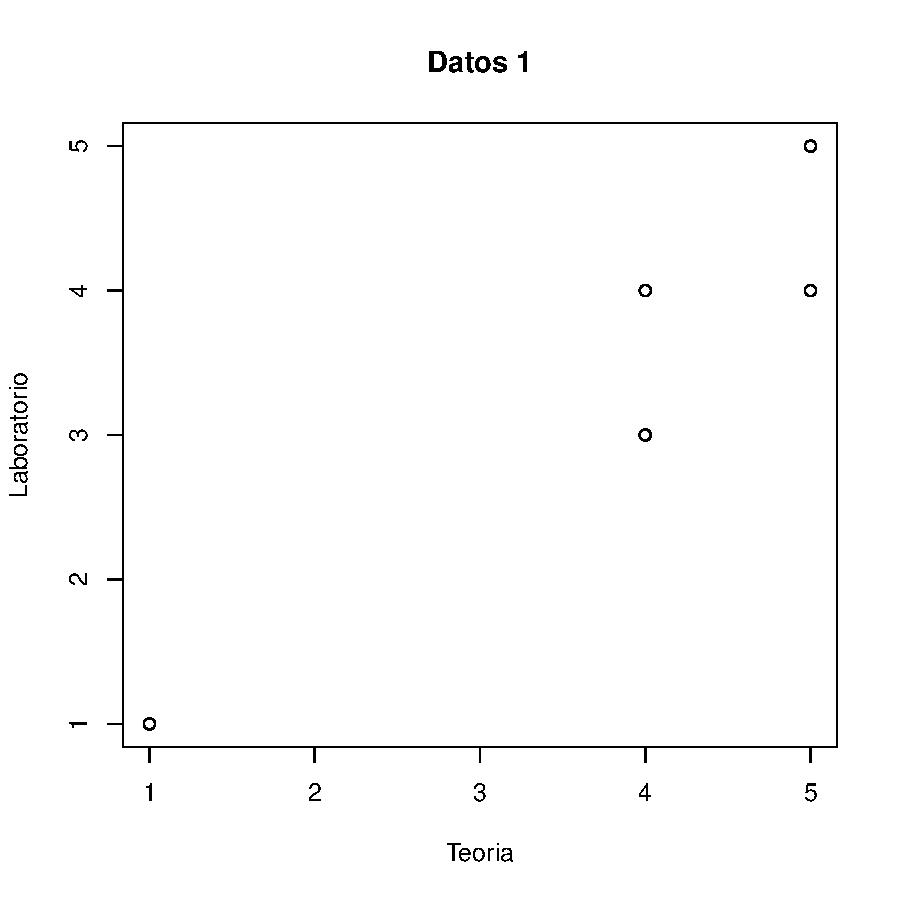
\includegraphics{entrega-plot_datos1}
\end{center}

\newpage
\subsubsection{Hormigón}
Los segundos representan la densidad y la resistencia del hormigón.
\begin{Schunk}
\begin{Sinput}
> datos2 <- data.frame(read.table("datos2.txt"))
> datos2
\end{Sinput}
\begin{Soutput}
  Resistencia Densidad
1         3.0      2.0
2         3.5     12.0
3         4.7      4.1
4         5.2      4.9
5         7.1      6.1
6         6.2      5.2
7        14.0      5.3
\end{Soutput}
\end{Schunk}
\begin{center}
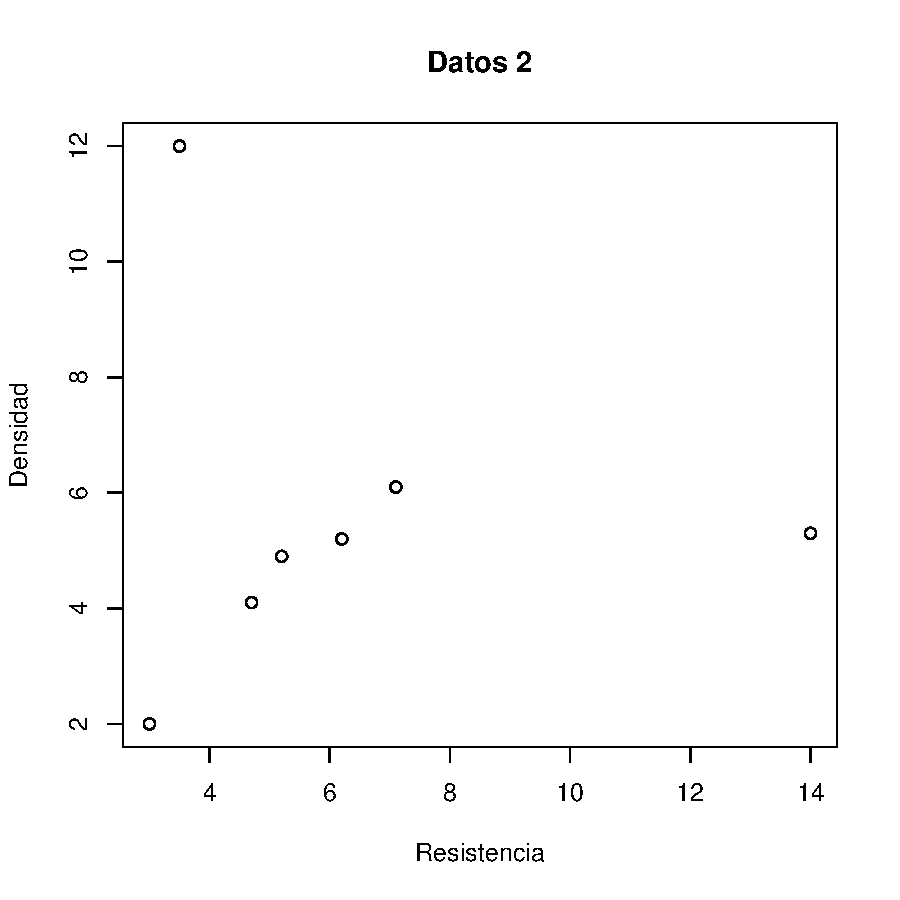
\includegraphics{entrega-plot_datos2}
\end{center}

\newpage
\subsection{K-vecinos sobre las notas para obtener outliers}
Aplicaremos el algoritmo k-vecinos sobre la muestra que tenemos.
Este algoritmo identificará de forma supervisada en la muestra datos anómalos, para poder obtener los outliers.

Calculamos las distancias euclídeas entre todos los puntos.
\begin{Schunk}
\begin{Sinput}
> distancias <- as.matrix(dist(datos1))
> distancias
\end{Sinput}
\begin{Soutput}
         1        2        3        4        5
1 0.000000 1.000000 1.414214 4.242641 1.000000
2 1.000000 0.000000 2.236068 3.605551 1.414214
3 1.414214 2.236068 0.000000 5.656854 1.000000
4 4.242641 3.605551 5.656854 0.000000 5.000000
5 1.000000 1.414214 1.000000 5.000000 0.000000
\end{Soutput}
\end{Schunk}

Elegimos el grado a partir del cual consideraremos que un pounto es outlier.
Todos los valores cuyo tercer vecino más cercano esté a una distancia superior a 2.5 los consideraremos outliers.
\begin{Schunk}
\begin{Sinput}
> max_radio <- 2.5
\end{Sinput}
\end{Schunk}

Mostramos en torno a cada valor un círculo con el radio indicado.
Si dentro del círculo dibujado no hay al menos otros tres datos dicho valor será considerado outlier.
Podemos ver que solo hay un punto para el que se da esta condición.
\begin{center}
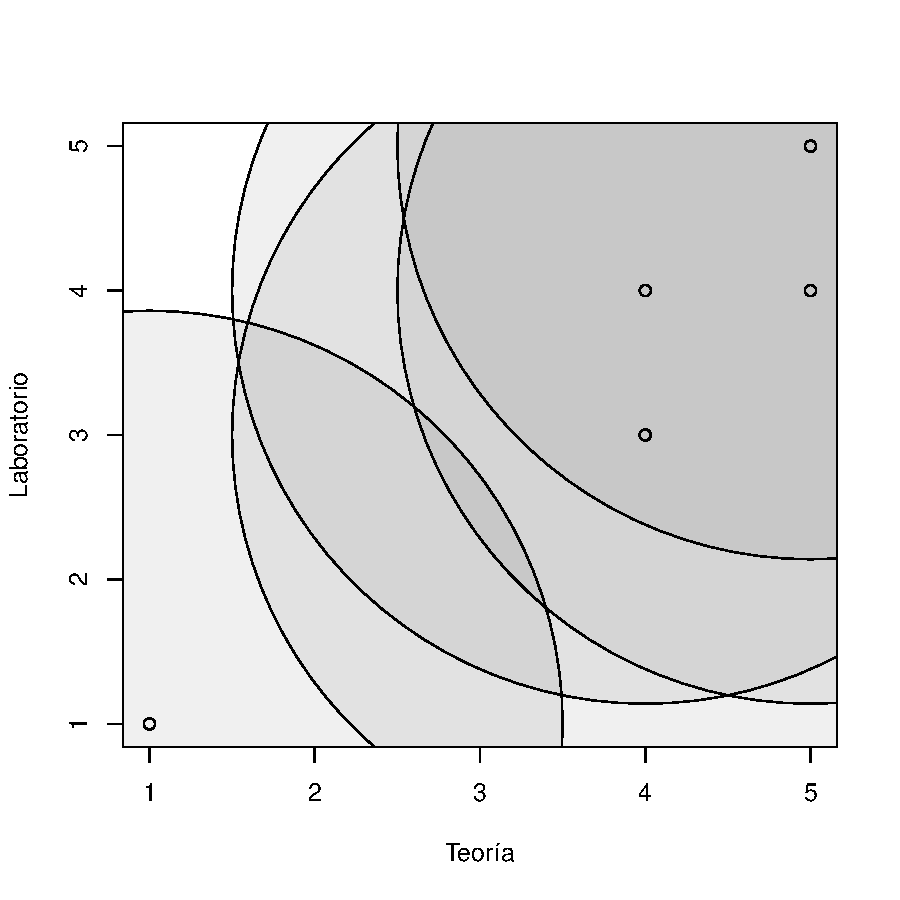
\includegraphics{entrega-k_vecinos_plot}
\end{center}

Calcularemos numéricamente ese valor.

Ordenamos las distancias de cada punto a todos los demás.
\begin{Schunk}
\begin{Sinput}
> for(i in 1:length(distancias[,1])){
+   distancias[,i] <- sort(distancias[,i])
+ }
> distanciasordenadas <- distancias
\end{Sinput}
\end{Schunk}

Reordenamos la matriz para organizarla en función de la distancia de cada punto a su vecino número 1,2,3...etc. 
Tras haber organizado la matriz, buscamos en el tercer vecino, que es el valor k que hemos usado en nuestro análisis para poder identificar los outliers.
\begin{Schunk}
\begin{Sinput}
> outliers_kvecinos = list()
> for(i in 1:length(distanciasordenadas[,1])){
+   if(distanciasordenadas[4,i]>max_radio){
+     outliers_kvecinos[[length(outliers_kvecinos)+1]] <- datos1[i,]
+   }
+ }
> outliers_kvecinos
\end{Sinput}
\begin{Soutput}
[[1]]
  Teoria Laboratorio
4      1           1
\end{Soutput}
\end{Schunk}

\newpage
\subsection{Deteccion de datos anómalos por cuartiles}
Sobre el segundo set de datos eliminaremos utilizando el método de los cuartiles.

Elegiremos el fator por el que multiplicar Q3-Q1.
Todos los valores que se alegen esa distancia de Q1 hacia los negativo o de Q3 hacia los positevos serán considerados outliers.
\begin{Schunk}
\begin{Sinput}
> max_range = 1.5
\end{Sinput}
\end{Schunk}

\subsubsection{Resistencia del hormigón}
Mostramos el diagrama de caja y bigotes de la resistencia.
\begin{center}
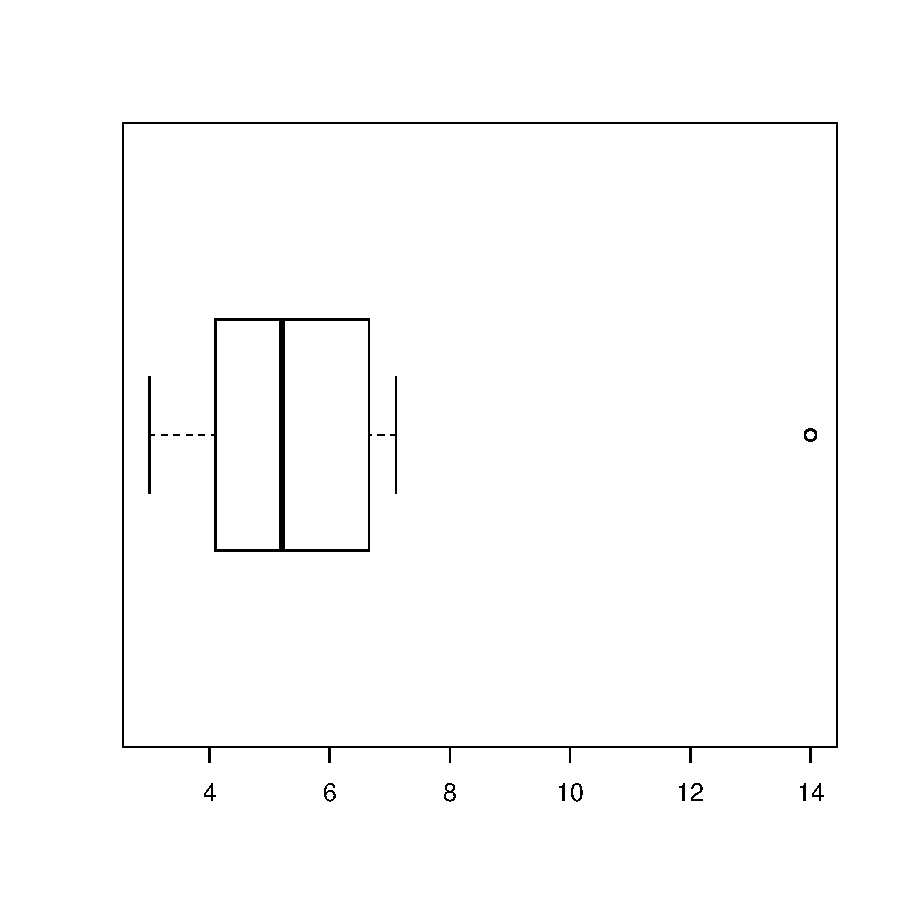
\includegraphics{entrega-plot_caja_bigotes_resistencia}
\end{center}

Calculamos ahora los valores que se salen del rango definido y que por tanto son outliers.
Para hacer esto primero obtenemos el intercalo de valores válidos
\begin{center}
\begin{Schunk}
\begin{Sinput}
> cuart1_res<-quantile(datos2$Resistencia,0.25)
> cuart3_res<-quantile(datos2$Resistencia,0.75)
> int_res=c(cuart1_res-max_range*(cuart3_res-cuart1_res),
+           cuart3_res+max_range*(cuart3_res-cuart1_res))
> int_res
\end{Sinput}
\begin{Soutput}
   25%    75% 
 0.275 10.475 
\end{Soutput}
\end{Schunk}
Ahora obtendremos los valores que quedan fuera de dicho intervalo.
\begin{Schunk}
\begin{Sinput}
> outliers_cuartiles_resistencia = list()
> for(i in 1:length(datos2$Resistencia)){
+   if(datos2$Resistencia[i]<int_res[1]||datos2$Resistencia[i]>int_res[2]){
+     outliers_cuartiles_resistencia[[length(outliers_cuartiles_resistencia)+1]] <- 
+         t(matrix(c(i, datos2[i,]$Resistencia), dimnames=list(c("Indice","Resistencia"))))
+   }
+ }
> outliers_cuartiles_resistencia
\end{Sinput}
\begin{Soutput}
[[1]]
     Indice Resistencia
[1,]      7          14
\end{Soutput}
\end{Schunk}
\end{center}
Como vemos el valor 12 es un outlier de la variable resistencia.

\subsubsection{Densidad del hormigón}
Repetimos este mismo análisis para la densidad.

Primero mostramos el diagrama de caja y bigotes para esta variable.
\begin{center}
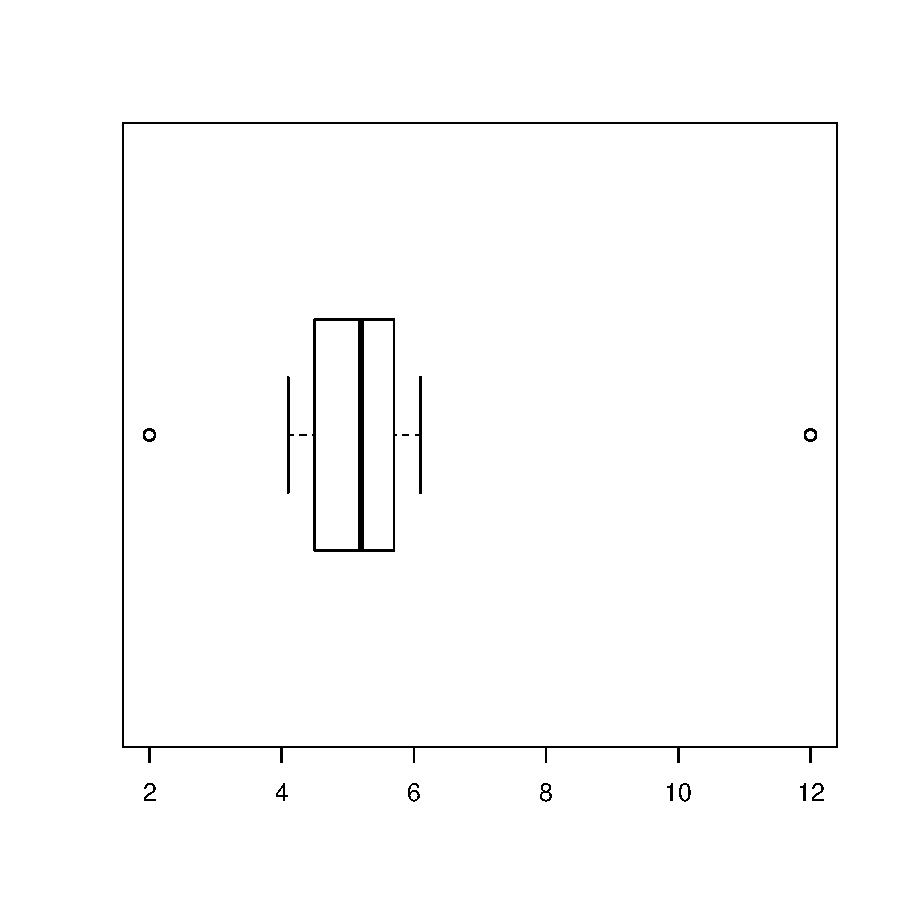
\includegraphics{entrega-plot_caja_bigotes}
\end{center}

Calculamos el intervalo a partir del que consideramos que los datos son outliers.
\begin{Schunk}
\begin{Sinput}
> cuart1_den<-quantile(datos2$Densidad,0.25)
> cuart3_den<-quantile(datos2$Densidad,0.75)
> int_dens=c(cuart1_den-max_range*(cuart3_den-cuart1_den), 
+            cuart3_den+max_range*(cuart3_den-cuart1_den))
> int_dens
\end{Sinput}
\begin{Soutput}
25% 75% 
2.7 7.5 
\end{Soutput}
\end{Schunk}

Obtenemos lo datos que quedan fuera del intervalo.
\begin{Schunk}
\begin{Sinput}
> outliers_cuartiles_densidad <- list()
> for(i in 1:length(datos2$Densidad)){
+   if(datos2$Densidad[i]<int_dens[1]||datos2$Densidad[i]>int_dens[2]){
+     outliers_cuartiles_densidad[[length(outliers_cuartiles_densidad)+1]] <- 
+       t(matrix(c(i, datos2[i,]$Densidad), dimnames=list(c("Indice","Densidad"))))
+   }
+ }
> outliers_cuartiles_densidad
\end{Sinput}
\begin{Soutput}
[[1]]
     Indice Densidad
[1,]      1        2

[[2]]
     Indice Densidad
[1,]      2       12
\end{Soutput}
\end{Schunk}
Esta vez hay dos valores outlier de densidad el 2 y el 12.

\newpage
\subsection{Outliers mediante la desviación típica}
Calcularemos los valores para cada que son considerados outliers por el método de la desviación tipica.
Dichos valores serán aquellos que se alejen demasidado de la media de la variable analizada.

En primer lugar elegiremos el factor por el que multiplicar la desviación típica para generar el intervalo de valores no outliers entorno a la media.
Metiante el teorema de tchebychev sabemos que para un valor de 2 al menos el 75\% de los datos estarán dentro del intervalo generado.
\begin{Schunk}
\begin{Sinput}
> max_deviation = 2
\end{Sinput}
\end{Schunk}

\subsubsection{Densidad del hormigón}
Mostramos la frecuencia realativa de la densidad del hormigón con respecto a la media de esta magnitud en azul.
En gris se muestra el intervalo a partir del cual los valores que queden fuera de él son considerados outliers.
\begin{center}
\begin{Schunk}
\begin{Sinput}
> plotFrecuencyData(datos2$Densidad)
\end{Sinput}
\end{Schunk}
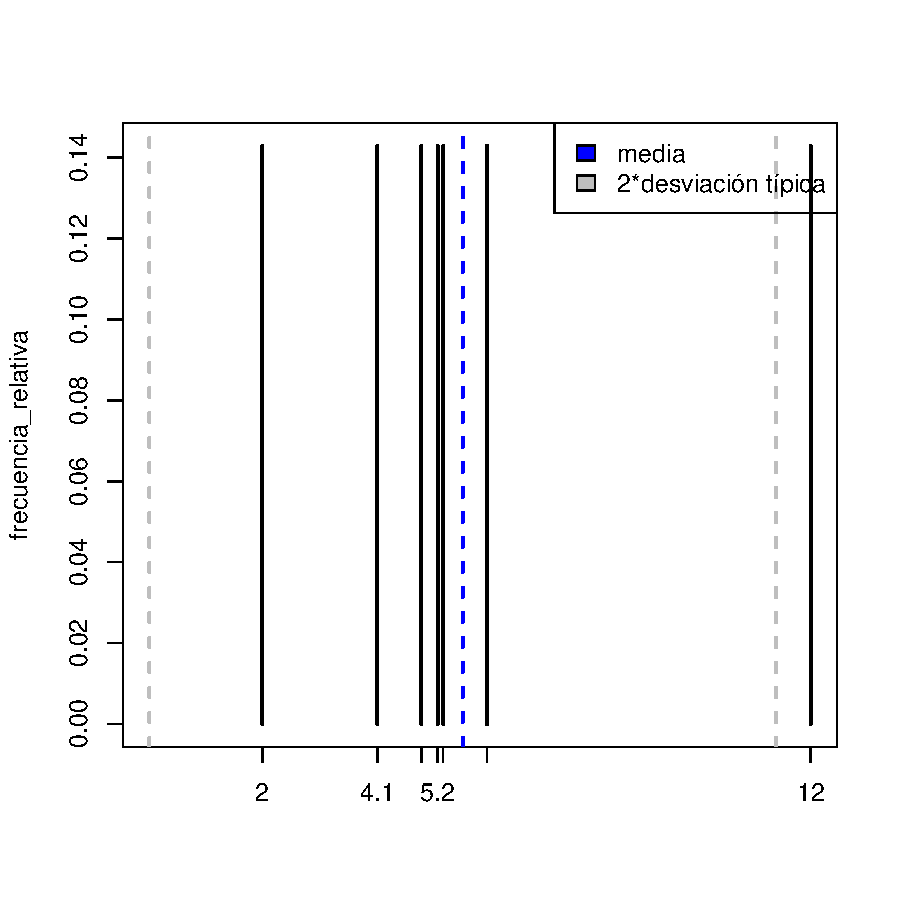
\includegraphics{entrega-desviacion_tipica_densidad_plot}
\end{center}

Ahora calculamos dichos valores.
Primero obtenemos el intervalo.
\begin{Schunk}
\begin{Sinput}
> int <- c(mediaAritmetica(datos2$Densidad) - 2*desviacionTipica(datos2$Densidad),
+          mediaAritmetica(datos2$Densidad) + 2*desviacionTipica(datos2$Densidad))
> int
\end{Sinput}
\begin{Soutput}
[1] -0.05685714 11.37114285
\end{Soutput}
\end{Schunk}
Podemos ver que el intervalo contiene valores de densidad irreales, esta no podría ser negativa.
En un anális de datos realista deberíamos corregir esto consultando con alguien que sea experto en los datos que estemos analizando.
Y luego los valores que quedan fuera de él.
\begin{Schunk}
\begin{Sinput}
> outliers_desviacion = list()
> for(i in 1:length(datos2$Densidad)) {
+   if ((datos2$Densidad[i]<int[1]) || (datos2$Densidad[i]>int[2])) {
+     outliers_desviacion[[length(outliers_desviacion)+1]] <- 
+       t(matrix(c(i, datos2[i,]$Densidad), dimnames=list(c("Indice","Densidad"))))
+   }
+ }
> outliers_desviacion
\end{Sinput}
\begin{Soutput}
[[1]]
     Indice Densidad
[1,]      2       12
\end{Soutput}
\end{Schunk}

\subsubsection{Resistencia del hormigón}
Mostramos la frecuencia realativa de la resistencia del hormigón con respecto a la media de esta magnitud en azul.
En gris se muestra el intervalo a partir del cual los valores que queden fuera de él son considerados outliers.
\begin{center}
\begin{Schunk}
\begin{Sinput}
> plotFrecuencyData(datos2$Resistencia)
\end{Sinput}
\end{Schunk}
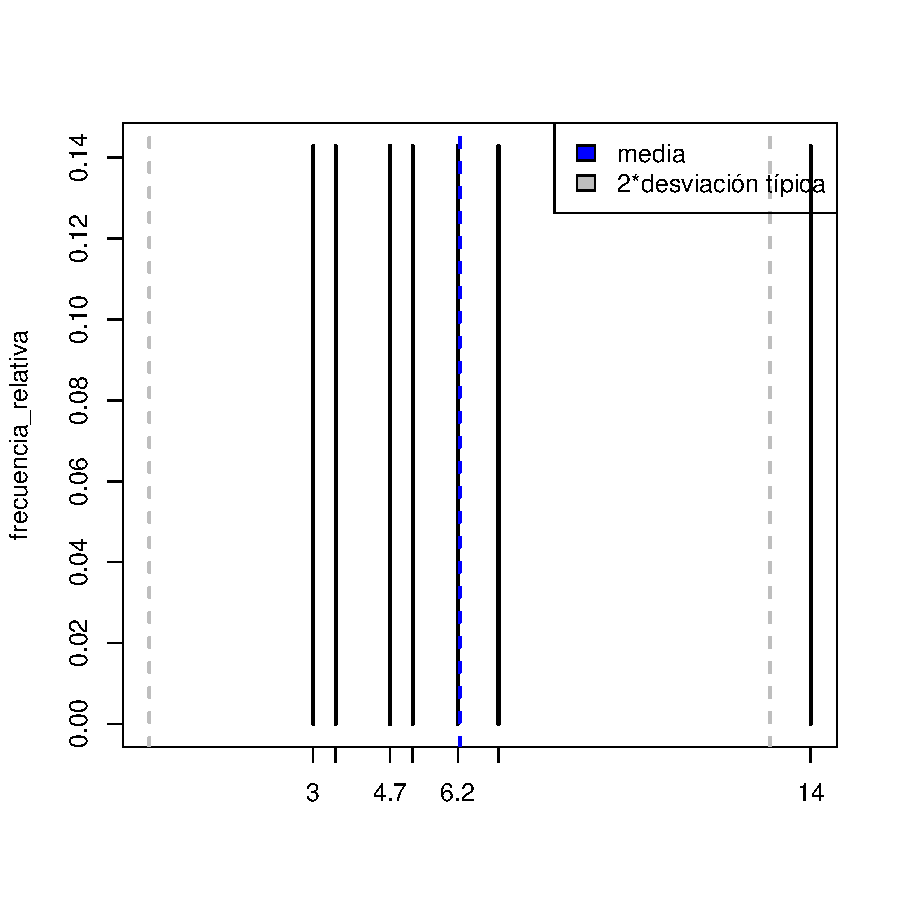
\includegraphics{entrega-desviacion_tipica_resistencia_plot}
\end{center}
Ahora calculamos dichos valores.
Primero obtenemos el intervalo.
\begin{Schunk}
\begin{Sinput}
> int <- c(mediaAritmetica(datos2$Resistencia) - 2*desviacionTipica(datos2$Resistencia), 
+          mediaAritmetica(datos2$Resistencia) + 2*desviacionTipica(datos2$Resistencia))
> int
\end{Sinput}
\begin{Soutput}
[1] -0.6197597 13.1054740
\end{Soutput}
\end{Schunk}
Podemos ver que el intervalo contiene valores de resistencia irreales, esta no podría ser negativa.
En un anális de datos realista deberíamos corregir esto consultando con alguien que sea experto en los datos que estemos analizando.
Y luego los valores que quedan fuera de él.
\begin{Schunk}
\begin{Sinput}
> outliers_desviacion = list()
> for(i in 1:length(datos2$Resistencia)) {
+   if ((datos2$Resistencia[i]<int[1]) || (datos2$Resistencia[i]>int[2])) {
+     outliers_desviacion[[length(outliers_desviacion)+1]] <- 
+       t(matrix(c(i, datos2[i,]$Resistencia), dimnames=list(c("Indice","Resistencia"))))
+   }
+ }
> outliers_desviacion
\end{Sinput}
\begin{Soutput}
[[1]]
     Indice Resistencia
[1,]      7          14
\end{Soutput}
\end{Schunk}

\newpage
\subsection{Detección de datos anómalos sobre la regresión de la densidad en función de la resistencia}

En este análisis detectamos los outliers utilizando la recta de regresión y el error estándar de los residuos.
Comenzaremos por determinar el factor por el que multiplicar el error estándar para considerar que los datos son outliers.
\begin{Schunk}
\begin{Sinput}
> sr_factor = 2
\end{Sinput}
\end{Schunk}

Comenzamos el análisis calculando la recta de regresión de los datos.
\begin{Schunk}
\begin{Sinput}
> dFr <- lm(datos2$Densidad~datos2$Resistencia)
\end{Sinput}
\end{Schunk}

Posteriormente, obtenemos los residuos calculados a partir de la recta de regresión y el error estándar.
\begin{Schunk}
\begin{Sinput}
> res <- summary(dFr)$residuals
> res
\end{Sinput}
\begin{Soutput}
         1          2          3          4          5          6          7 
-3.8427477  6.1858698 -1.6454482 -0.8168308  0.4919157 -0.4595958  0.0868370 
\end{Soutput}
\begin{Sinput}
> sr <- sqrt(sum(res^2)/length(res))
> sr
\end{Sinput}
\begin{Soutput}
[1] 2.850242
\end{Soutput}
\end{Schunk}

A partir del error estándar y de la recta de regresión obtenida podremos mostrar los datos junto a su recta de regresión.
Paralela a dicha recta mostramos otras dos que marcan la frontera a partir de la que los valores se considerarán outliers.
En este caso solo se ve la recta paralela superior.
\begin{center}
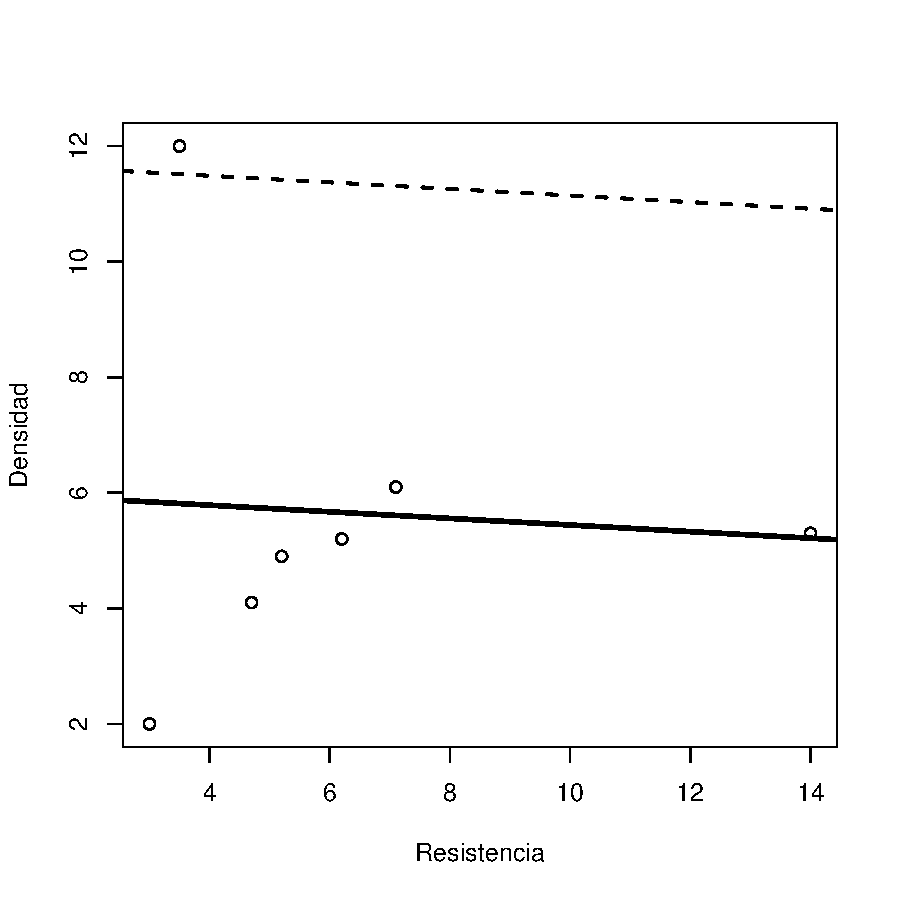
\includegraphics{entrega-regresion_plot}
\end{center}

Con el error estándar de los residuos, comparamos cada uno para comprobar si es mayor que el error estándar multiplicado por el factor establecido.
Si se da el caso, podemos considerar ese punto como un outlier.
\begin{Schunk}
\begin{Sinput}
> outliers_regresion = list()
> for(i in 1:length(res)){
+   if(abs(res[i])>sr_factor*sr){
+     outliers_regresion[[length(outliers_regresion)+1]] <- datos2[i,]
+   }
+ }
> outliers_regresion
\end{Sinput}
\begin{Soutput}
[[1]]
  Resistencia Densidad
2         3.5       12
\end{Soutput}
\end{Schunk}

\newpage
\section{Anális de outliers en datos climáticos}

Realizaremos un anális de outliers sobre un conjunto de datos en que que hay las siguientes variables.
Mes en el que se capturaron los datos, cantidad de ozono, presión, velocidad del viento, humedad, visibilidad y temperatura de dos sensores distintos.

A lo largo del análisis podemos ver que la muestra de datos carece de valores outlier que sean notables.
No obstante aunque esta haya sido la conclusión finalmente obtenida debe ser necesario mencionar que es una conclusión válida.

\begin{Schunk}
\begin{Sinput}
> datos3 <- read.csv("ozone.csv")
\end{Sinput}
\end{Schunk}

\subsection{Outliers por cuartiles en cada mes}

Deseamos ver si hay algún dato cuya humedad sea inusualmente alta o baja para la que debería de estar sucediendo cuando fue capturado.
Para ello trateremos las medidas de la humedad clasificadas por meses.
Entendemos que las medidas de un mismo mes debería de ser relativamente homogéneas.

Elegimos el factor a partir del cual calcular el intervalo de valores válidos para el análisis por cuartiles.
\begin{Schunk}
\begin{Sinput}
> cuartiles_factor = 1.5
\end{Sinput}
\end{Schunk}

Mostramos el diagrama de caja y bigotes de los datos de la humedad agrupados por mes.

En él podemos realizar dos observaciones.
Solo en algunos meses, los más próximos la verano, los datos tienen un rango de variación reducido.
Por el contrario en otros meses, lo más próximos al invierno, se registran valores de humedad en un rango mayor.

Será por tanto que solo en los meses con un rango reducido podremos obtener outliers.
En estos meses ciertos rangos humedad son mucho más frecuentes que otros.
Aquellos valores que se alejen de los intervalos de cuartiles serán outliers y tendrán especial relevancia pues informarán sobre anomalías en la humedad en los días en los que se produjero.
Estos serán días inusualmente secos o inusualmente húmedos.

\begin{center}
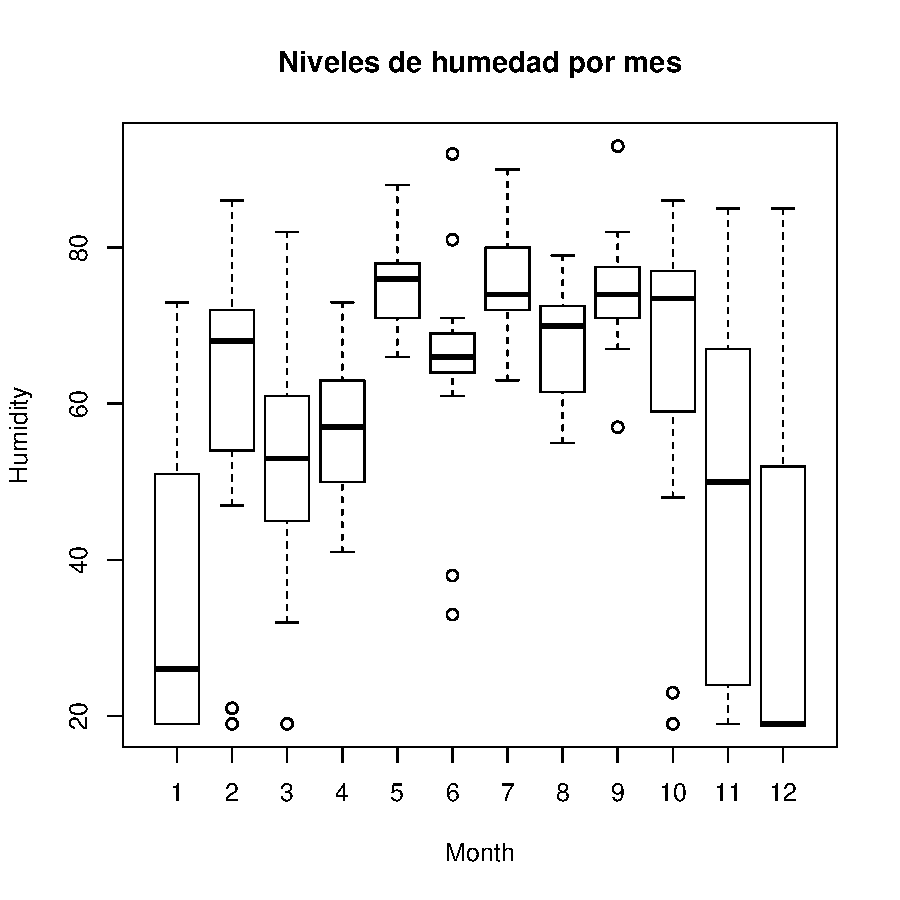
\includegraphics{entrega-datos_humedad_mes_cuart}
\end{center}

Filtramos los datos originales indicando si sus niveles de humedad se salen del rango de curtiles de su mes.
\begin{Schunk}
\begin{Sinput}
> vectoroutliers<- vector(mode="numeric", length=0)
> for(mes in 1:12){
+   mes_data <- subset(datos3,datos3$Month==mes)
+   cuar1 <- quantile(mes_data$Humidity,0.25)
+   cuar3 <- quantile(mes_data$Humidity,0.75)
+   int <- c(cuar1-cuartiles_factor*(cuar3-cuar1), cuar3+cuartiles_factor*(cuar3-cuar1))
+   for(i in 1:length(mes_data$Humidity)){
+     vectoroutliers <- c(vectoroutliers, 
+       (mes_data$Humidity[i]<int[1])||(mes_data$Humidity[i]>int[2]))
+   }
+ }
> datos_filtrados_cuartiles=cbind(vectoroutliers,datos3)
> datos_filtrados_cuartiles=subset(datos_filtrados_cuartiles,
+   datos_filtrados_cuartiles[,1]==0)
> datos_outliers_cuartiles=cbind(vectoroutliers,datos3)
> datos_outliers_cuartiles=subset(datos_outliers_cuartiles,
+   datos_outliers_cuartiles[,1]==1)
> length(datos_outliers_cuartiles)
\end{Sinput}
\begin{Soutput}
[1] 14
\end{Soutput}
\end{Schunk}

Finalmente mostramos aquellos valores que han sido considerados outliers dibujados en rojo.
\begin{center}
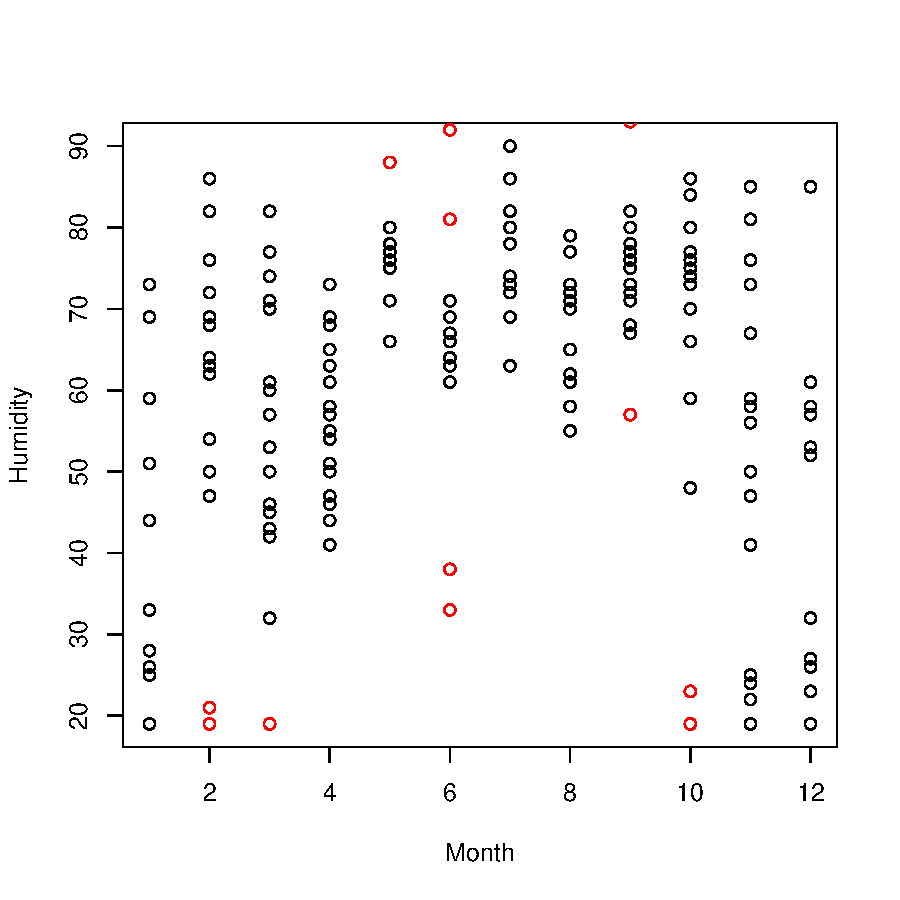
\includegraphics{entrega-datos_humedad_mes_filtrados}
\end{center}

\newpage
\subsection{Diferencia de temperatura en los sensores}

A continuación calcularemos la regresión entre las medidas de temperatura capturadas con dos sensores distintos ubicados en localidades próximas.
Las medidas de ambos deberían de ser muy parecidad pues las localidades no están suficiéntemente alejadas.

Aquellos valores que se alejen demasiado de la recta de regresión podrán indicar error en la medida realizada por alguno de los sensores.
Otra cosa que podrían revelar estos outliers son episidios de microclima que pudieran darse solo en una de las localidades.

Elegimos el valor a partir del que queramos considerar outlier a los datos.
\begin{Schunk}
\begin{Sinput}
> regresion_factor = 2.5
\end{Sinput}
\end{Schunk}

Mostramos la regresión entre las temperaturas de ambos sensores.
\begin{center}
\begin{Schunk}
\begin{Sinput}
> dFr <- lm(datos3$Temperature_Sandburg~datos3$Temperature_ElMonte)
> res <- summary(dFr)$residuals
> sr <- sqrt(sum(res^2)/length(res))
> regPlot (datos3$Temperature_ElMonte, datos3$Temperature_Sandburg, dFr, 
+           sr*regresion_factor, xlabel="Temperatura ElMonte",
+                                ylabel="Temperature Sandburg")
\end{Sinput}
\end{Schunk}
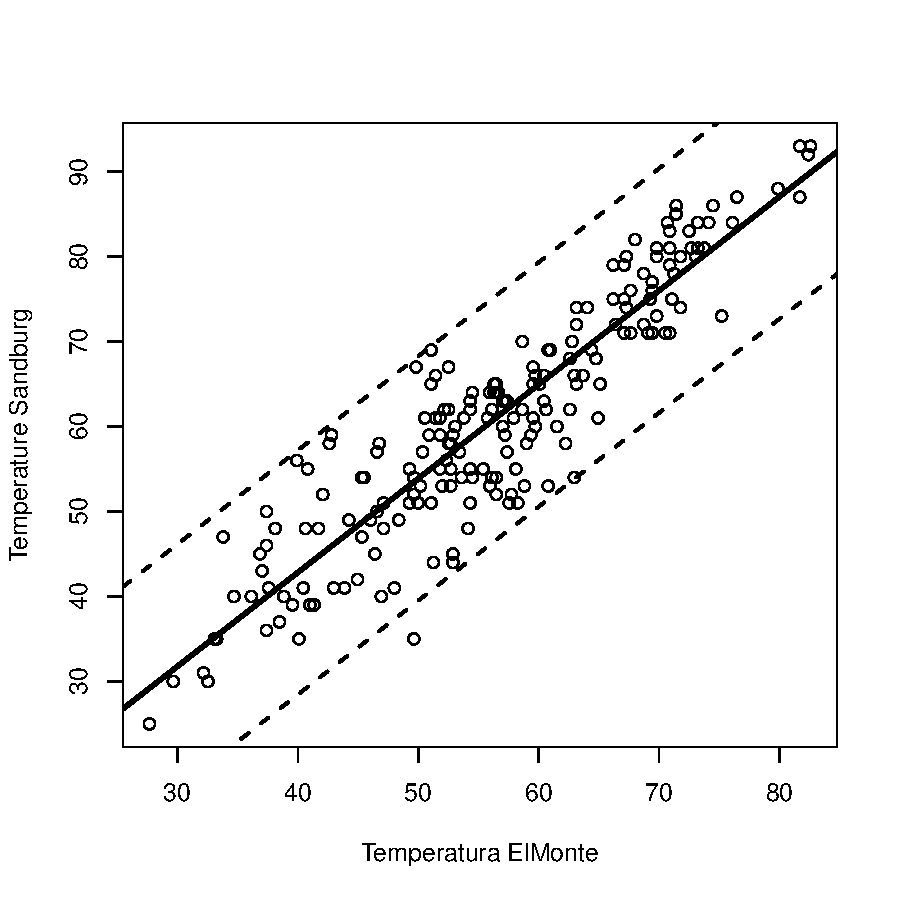
\includegraphics{entrega-temp_plot}
\end{center}
Como podemos ver ambas medidas están muy correladas.
\begin{Schunk}
\begin{Sinput}
> summary(dFr)$r.squared
\end{Sinput}
\begin{Soutput}
[1] 0.8353271
\end{Soutput}
\end{Schunk}

Solo un valor es finalmente considerado outlier.
Debido a que este valor es único y que tampoco aparece demasiado alejado del resto puede que realmente no lo sea.
\begin{Schunk}
\begin{Sinput}
> vectoroutliers<- vector(mode="numeric", length=0)
> for(i in 1:length(res)){
+     vectoroutliers <- c(vectoroutliers, abs(res[i])>regresion_factor*sr)
+ }
> datos_filtrados_regresion <- cbind(vectoroutliers,datos3)
> datos_filtrados_regresion <- subset(datos_filtrados_regresion,
+   datos_filtrados_regresion[,1]==0)
> datos_outliers_regresion <- cbind(vectoroutliers,datos3)
> datos_outliers_regresion <- subset(datos_outliers_regresion,
+   datos_outliers_regresion[,1]==1)
> length(datos_outliers_regresion)
\end{Sinput}
\begin{Soutput}
[1] 14
\end{Soutput}
\end{Schunk}

Mostramos ahora los outliers en rojo junto a los datos originales
\begin{center}
\begin{Schunk}
\begin{Sinput}
> plot(datos_filtrados_regresion$Temperature_ElMonte,
+     datos_filtrados_regresion$Temperature_Sandburg,
+     xlab="Temperatura ElMonte",ylab="Temperature Sandburg")
> points(datos_outliers_regresion$Temperature_ElMonte, 
+     datos_outliers_regresion$Temperature_Sandburg, col="red")
\end{Sinput}
\end{Schunk}
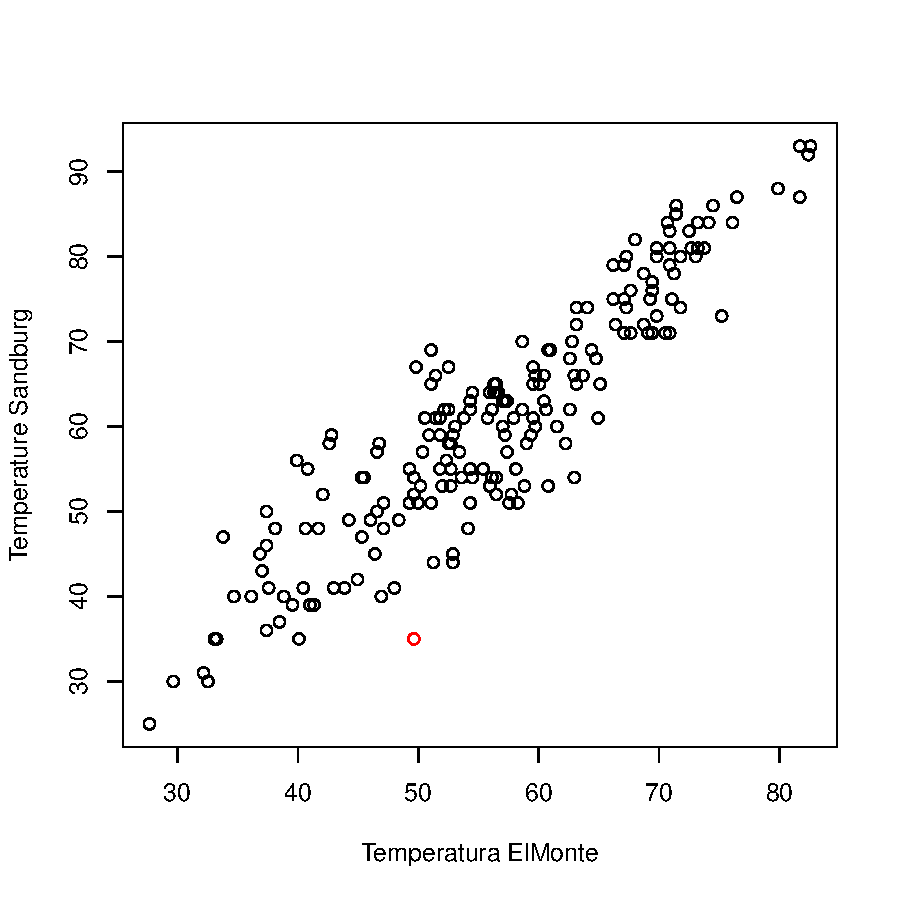
\includegraphics{entrega-temp_filter}
\end{center}

\newpage
\section{Anális outliers en datos de incendios}
Tenemos una muestra de datos de la humedad, temperatura, velocidad del viento, cantidad de lluvia y área quemada de distintos incendios.
Sobre dicha muestra realizaremos un análisis de outliers utilizando las variables de la temperatura y la humedad con respecto al área quemada.

Ya que queremos utilizar tres variables para el análisis muchos de los métodos estudiados no podrán ser usados.
La mayoría como la desviación típica o los cuartiles son solo sobre una variable. La correlación por el contrarios es solo sobre dos.

Utilizaremos por tanto las local features y la distancia de mahalanobis, dos métodos capaces de buscar outliers sobre n-dimensiones.
Mostraremos los datos utilizando "scatterplot3d" capaz de crear gráficas tridimensionales.

Primero deberemos cargar y normalizar la muestra de datos.
\begin{center}
\begin{Schunk}
\begin{Sinput}
> data <- read.csv("forestfires.csv")
> data <- data[,c(9,10, 13)]
> data <- na.omit(data)
> normalize <- function(x){
+   return ((x-min(x))/(max(x)-min(x)))
+ }
> data <- as.data.frame(lapply(data[,c(1,2,3)],normalize))
> scatterplot3d(data$temp, data$RH, data$area)
\end{Sinput}
\end{Schunk}
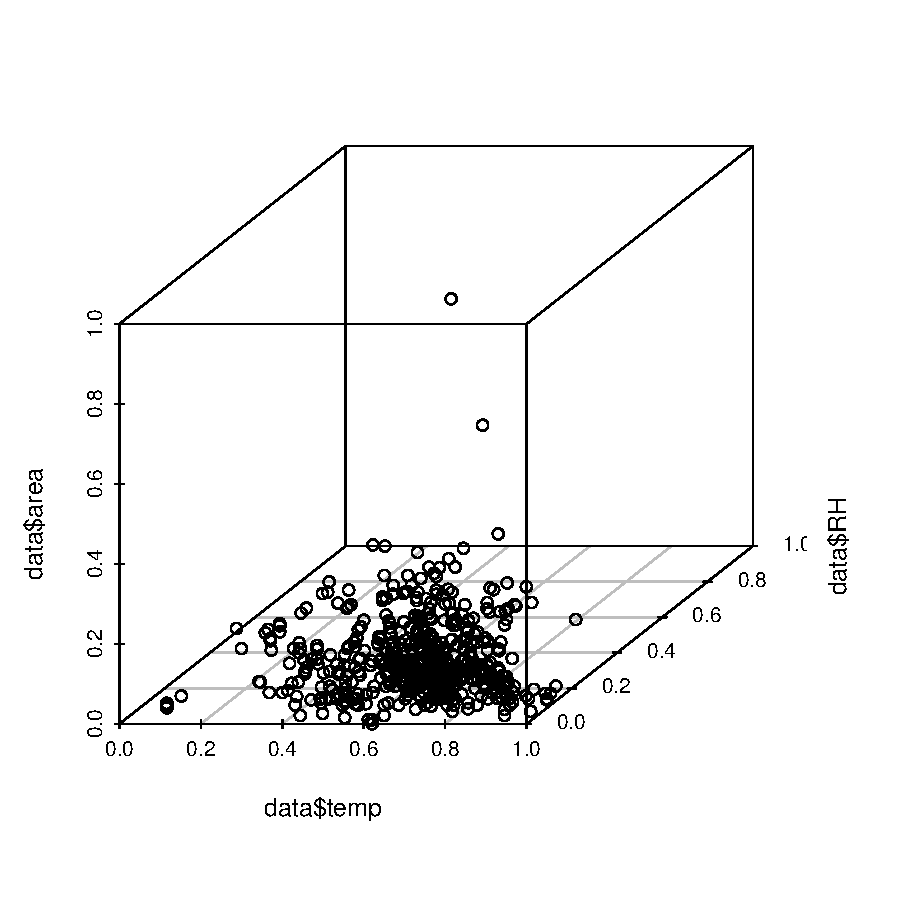
\includegraphics{entrega-forest_fires_data}
\end{center}

\subsection{Outliers por Local Features}
Buscaremos ahora outliers utilizando local features del paquete "Rlof".
Esta técnica utilizar k-vecinos para encontrar outlier por densidad.
Nos proporciona una puntución para cada dato de la muestra en función de la cual podremos determinar si dicho punto es o no outlier.
Tendrán mayor puntución aquellos valores que estén muy alejados del resto, es decir, que tengan pocos vecinos a su alrededor y que estén lejos de ellos.

Consideraremos que son outliers datos a una distancia mayor de 2.5 de su cuarto vecino más próximo.
Consideraremos por tanto que tres puntos cercanos forman un cluster.
\begin{Schunk}
\begin{Sinput}
> umbral <- 2.5
> data$score<-lof(data, k=3)
> data$outlier <- (data$score>umbral)
\end{Sinput}
\end{Schunk}

Mostramos los resultados.
\begin{center}
\begin{Schunk}
\begin{Sinput}
> data$color <- ifelse(data$outlier, "red", "black")
> scatterplot3d(data$temp, data$RH, data$area, color = data$color)
\end{Sinput}
\end{Schunk}
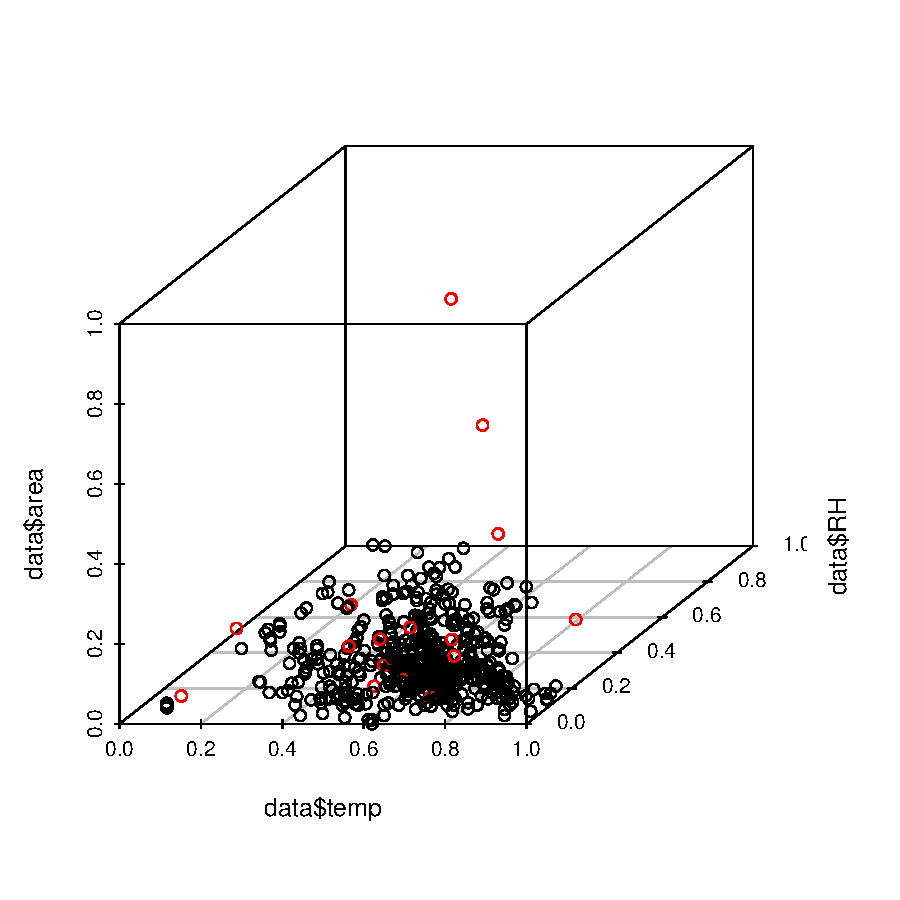
\includegraphics{entrega-display}
\end{center}

Se consideran outliyer puntos con humedades y temperaturas muy bajas o altas y también puntos con áres quemadas muy elevadas.
Podemos ver también que la representación tridimensional no es demasiado precisa ya que vemos una proyección bidimensional de esta.
Solo con la representación tridimensional nos es difícil saber que puntos han sido considerados outliers.
\begin{center}
\begin{Schunk}
\begin{Sinput}
> subset(data[c(1,2,3,4)],data$outlier==1)
\end{Sinput}
\begin{Soutput}
          temp        RH        area    score
2   0.50803859 0.2117647 0.000000000 2.635202
78  0.19614148 0.6705882 0.000000000 2.513442
120 0.55948553 0.2470588 0.000000000 2.888904
226 0.66559486 0.2823529 0.044506985 3.141092
230 0.45659164 0.3294118 0.065362473 2.511093
233 0.53054662 0.3294118 0.094780169 2.502027
235 0.49839228 0.1176471 0.141982326 3.970820
239 0.73633441 0.1411765 1.000000000 3.593839
281 0.00000000 0.5176471 0.008498038 2.529936
282 0.09324759 0.1058824 0.022707271 3.903732
330 0.68488746 0.1411765 0.003052693 3.167307
333 0.47909968 0.3058824 0.010285651 2.638249
393 0.63344051 0.3294118 0.064867442 2.810302
416 0.81350482 0.1411765 0.684133328 3.065509
480 0.65594855 0.4941176 0.255335338 2.545245
500 0.80707395 0.5647059 0.009918962 4.853120
\end{Soutput}
\end{Schunk}
\end{center}

\newpage
\subsection{Outliers por distancia de Mahalanobis}
Buscaremos outlier utilizando la distancia de mahalanobis.
Esta métrica tiene es una mejora sobre la distancia estadística o de Gauss en la que se tiene en cuenta la correlación de las variables.
La ventaja de este método respecto del anterior es que no podemos obtener una detección de outliers peor por haber indicado un número de vecinos demasiado alto o bajo.
Se utilizar para detectarlos la correlación que en algunos casos puede ser mejor.

Consideraremos que son outliers datos con distancia de mahalanobis mayor que 8.
\begin{Schunk}
\begin{Sinput}
> umbral <- 8
> data$mahalanobis <- mahalanobis(data[,1:3], colMeans(data[,1:3]), cov(data[,1:3]))
> data <- data[order(data$mahalanobis,decreasing = TRUE),]
> data$outlier <- (data$mahalanobis>umbral)
\end{Sinput}
\end{Schunk}

Mostramos los resultados.
Podemos ver que mucho puntos coinciden con los calculados por k-vecinos.
\begin{center}
\begin{Schunk}
\begin{Sinput}
> data$color <- ifelse(data$outlier, "red", "black")
> scatterplot3d(data$temp, data$RH, data$area,  color = data$color)
\end{Sinput}
\end{Schunk}
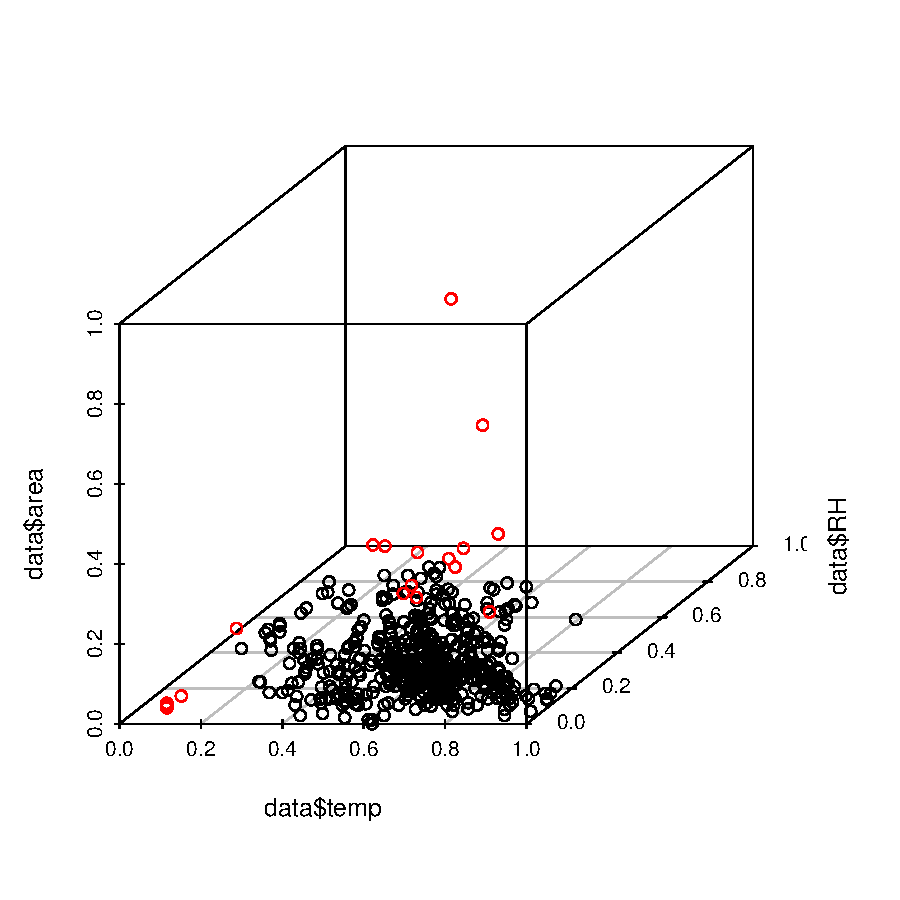
\includegraphics{entrega-mahalanobis_plot}
\end{center}

\newpage
\section{Clasificación supervisada con K-vecinos}
Deseamos probar el algoritmo k-vecinos visto como un método para encontrar outliers esta vez aplicado a clasificación supervisada.
Proporcionaremos un conjunto de datos de los que ya conocemos su clasificación y a partir de ellos crearemos un clasificador knn.
La muestra utilizada se corresponden con medidas realizadas sobre distintos tipos de flores.
Se miden los pétalos y los sépalos y se clasifican en 3 categorías: setosa, versicolor y virginica.

Antes de utilizar los datos será necesario normalizarlos.
\begin{Schunk}
\begin{Sinput}
> data("iris")
> normalize <- function(x){
+   return ((x-min(x))/(max(x)-min(x)))
+ }
\end{Sinput}
\end{Schunk}

Para validar el clasificador utilizaremos la mitad de los datos de los que disponemos como datos de "entrenamiento" siendo la otra mitad datos de "test".
Para elegir la mitad de los datos desordenaremos previamente estos de modo que en cada conjunto pueda haber datos de todo tipo.
\begin{Schunk}
\begin{Sinput}
> rnum<- sample(rep(1:length(iris[,1])))
> iris<- iris[rnum,]
> iris.new<- as.data.frame(lapply(iris[,c(1,2,3,4)],normalize))
> train_limit <- floor(length(iris[,1])*0.5)
> iris.train <- iris.new[1:train_limit,]
> iris.train.target<- iris[1:train_limit,5]
> iris.test <- iris.new[(train_limit+1):length(iris[,1]),]
> iris.test.target <- iris[(train_limit+1):length(iris[,1]),5]
\end{Sinput}
\end{Schunk}

Creamos tres clasificadores disntintos teniendo en cuenta 1, 8 y 16 vecinos respectivamente.
\begin{Schunk}
\begin{Sinput}
> modelknn1 <- knn(train=iris.train, test=iris.test, cl=iris.train.target, k=1)
> modelknn8 <- knn(train=iris.train, test=iris.test, cl=iris.train.target, k=8)
> modelknn16 <- knn(train=iris.train, test=iris.test, cl=iris.train.target, k=16)
\end{Sinput}
\end{Schunk}

Finalmente evaluamos la calidad de la clasificación obtenida creando matrices de confusión para cada uno de los clasificadores.
En este caso lo resultados son muy similares en los tres, pero esto podría no ser así.
Podemos ver que el clasificador acirta en la mayoría de los casos.
Se puede ver también que el clasificador parece tener problemas para distinguir entre virginica y versicolor.
Suelen aparecer errores cruzados entre esas dos clases, aunque ello depende de la elección aleatoria de los datos de test y entrenemiento.
\begin{Schunk}
\begin{Sinput}
> table(iris.test.target, modelknn1)
\end{Sinput}
\begin{Soutput}
                modelknn1
iris.test.target setosa versicolor virginica
      setosa         25          0         0
      versicolor      0         24         2
      virginica       0          2        22
\end{Soutput}
\begin{Sinput}
> table(iris.test.target, modelknn8)
\end{Sinput}
\begin{Soutput}
                modelknn8
iris.test.target setosa versicolor virginica
      setosa         25          0         0
      versicolor      0         25         1
      virginica       0          1        23
\end{Soutput}
\begin{Sinput}
> table(iris.test.target, modelknn16)
\end{Sinput}
\begin{Soutput}
                modelknn16
iris.test.target setosa versicolor virginica
      setosa         25          0         0
      versicolor      0         26         0
      virginica       0          3        21
\end{Soutput}
\end{Schunk}

\newpage
\section{Funciones utilizadas}
Mostramos las funciones utilizadas para crear las gráficas de regresión mostrando los límites a partir de las que consideramos que un valor es outlier y la gráfica para considerar outliiers por desviación típica.
\begin{Schunk}
\begin{Sinput}
> regPlot
\end{Sinput}
\begin{Soutput}
function (x, y, regresion, limit, xlabel="", ylabel="") {
  plot(x, y, xlab=xlabel, ylab=ylabel)
  regUpLimit <- regresion
  regUpLimit$coefficients[1] = regUpLimit$coefficients[1] + limit
  regDownLimit <- regresion
  regDownLimit$coefficients[1] = regDownLimit$coefficients[1] - limit
  abline(regUpLimit, "gray", lty=2, lwd=2)
  abline(regresion, "black", lty=1, lwd=3)
  abline(regDownLimit, "gray", lty=2, lwd=2)
}
<bytecode: 0x7fd09169b1b8>
\end{Soutput}
\begin{Sinput}
> plotFrecuencyData
\end{Sinput}
\begin{Soutput}
function(data, xlabel="") {
  uniquedata<-unique(data)
  frecuencia_relativa <- as.table(frecuenciaRelativa(data))
  media_ <- mediaAritmetica(data)
  desviacion_tipica_ <- desviacionTipica(data)
  tchebychev_min <- media_-2*desviacion_tipica_
  tchebychev_max <- media_+2*desviacion_tipica_
  min_range = min(tchebychev_min, min(uniquedata))
  max_range = max(tchebychev_min, max(uniquedata))
  plot(frecuencia_relativa, type="h", xlab=xlabel, xlim=c(min_range,max_range))
  abline (v=c(media_, tchebychev_min, tchebychev_max), 
          col=c("blue", "gray", "gray"), lty=c(2,2,2,3,3),
          lwd=c(2,2,2,1,1))
  legend ("topright", legend=c("media", "2*desviación típica"),
          fill=c("blue","gray"))
}
<bytecode: 0x7fd093eb38e8>
\end{Soutput}
\end{Schunk}

\end{document}
